\documentclass{article}
\usepackage{graphicx} % Required for inserting images
\usepackage[top=0.9in, bottom=1in, left=1.5in, right=1.5in]{geometry}
\usepackage[utf8]{inputenc}
\usepackage[icelandic]{babel}
\usepackage[T1]{fontenc}
\usepackage[sc]{mathpazo}
\usepackage[parfill]{parskip}
\renewcommand{\baselinestretch}{1.2}
% Tables and lists
\usepackage{booktabs,tabularx}
\usepackage{multirow}
\usepackage{enumerate}
\usepackage{adjustbox}
\usepackage{multicol}
\usepackage{xcolor}
\usepackage{algpseudocode}
\usepackage{tikz}
\usepackage{nicefrac}
\usepackage{changepage}
\usetikzlibrary{arrows, positioning, calc, graphs}

% Math
\usepackage{amsmath, amsfonts, amssymb, amsthm}
% Graphics

\usepackage{graphicx}
\usepackage{tikz}
% Code environment
\usepackage{minted}
%\usepackage{bm}
%\usepackage{siunitx}
%\usepackage{animate}
%\usepackage{hyperref}
%\usepackage{movie15}
%\usepackage{multicol}
%\usepackage{changepage}
\title{Forritunarmál Einstaklingsverkefni 6}
\author{Ragnar Björn Ingvarsson, rbi3}
\tikzset{->, >=stealth', shorten >=1pt, node distance=2cm,thick, main node/.style={circle,draw,minimum size=3em}}

\begin{document}
\renewcommand\thepage{}
	
	\maketitle

	\newpage
	\setcounter{page}{1}
	\renewcommand\thepage{\arabic{page}}

	\section{}
	\begin{verbatim}
(*
Notkun: lengd x
Fyrir: x er listi gilda af hvaða tagi sem er, x=[x1;...;xn]
Gildi: Fjöldi staka í listanum
*)
let lengd x =
    list_it (fun _ y -> 1+y) x 0
;;
	\end{verbatim}
	\begin{center}
		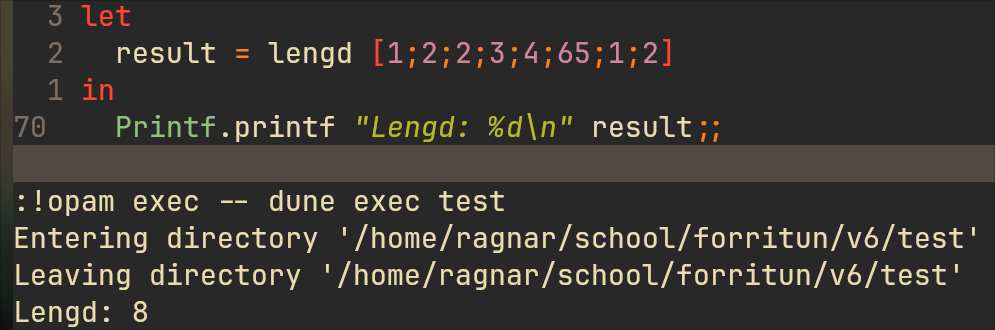
\includegraphics[scale=0.35]{lengd.png}
	\end{center}
	\begin{center}
		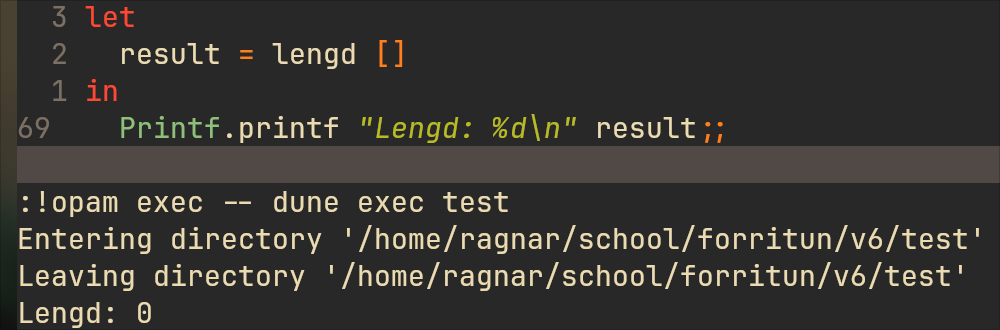
\includegraphics[scale=0.35]{lengd2.png}
	\end{center}

	\newpage
	\section{}
	\begin{verbatim}
(*
Notkun: powerList x
Fyrir: x er listi, x=[x1;x2;...;xn]
Gildi: Listi allra mögulegra lista sem eru undirlistar
       listans x. Fjöldi staka er þá 2^n
*)
let rec powerList x =
    match x with
      [] -> 
        [[]]
    | 
      x::xs ->
        let rest = powerList xs
        in 
          rest @ List.map (fun l -> x::l) rest
;;
	\end{verbatim}

	Og hér eru prent-hjálparföllin

	\begin{verbatim}
(*
Notkun: print_list l
Fyrir: l er listi af heiltölum, l=[l1;l2;...;ln]
Gildi: Ekkert skilagildi en prentar "[l1; l2; ...; ln; ]"
*)
let print_list l = 
  print_string "[";
  List.iter (fun x -> print_int x; print_string "; ") l;
  print_string "]"
;;

(*
Notkun: print_power_list pl
Fyrir: pl er listi af listum af heiltölum, 
       [[pl11;pl12;...;pl1n];[pl21;...;pl2n];...;[plm1;...;plmn]]
Gildi: Ekkert skilagildi en prentar 
       "[[pl11; ...; pl1n; ]; ...; [plm1; ...; plmn; ]; ]" og nýja línu
*)
let print_power_list pl =
  print_string "[";
  List.iter (fun l -> print_list l; print_string "; ") pl;
  print_string "]\n"
;;
	\end{verbatim}
	\begin{center}
		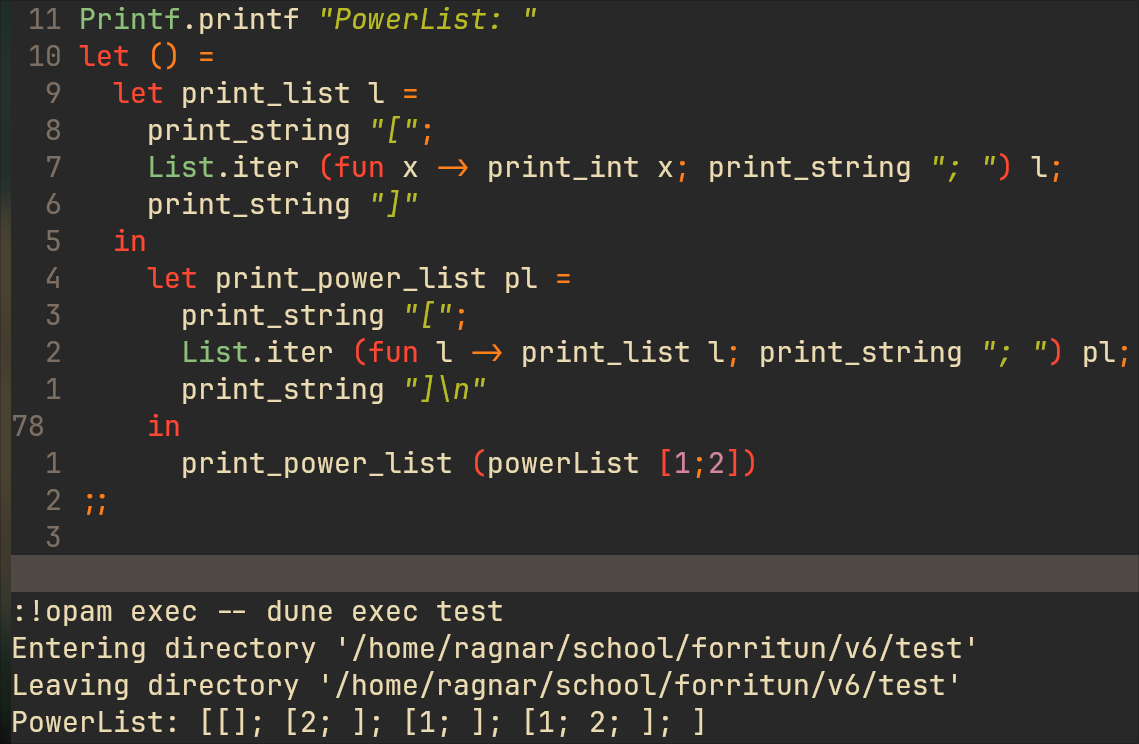
\includegraphics[scale=0.3]{powerlist.png}
	\end{center}
	\begin{center}
		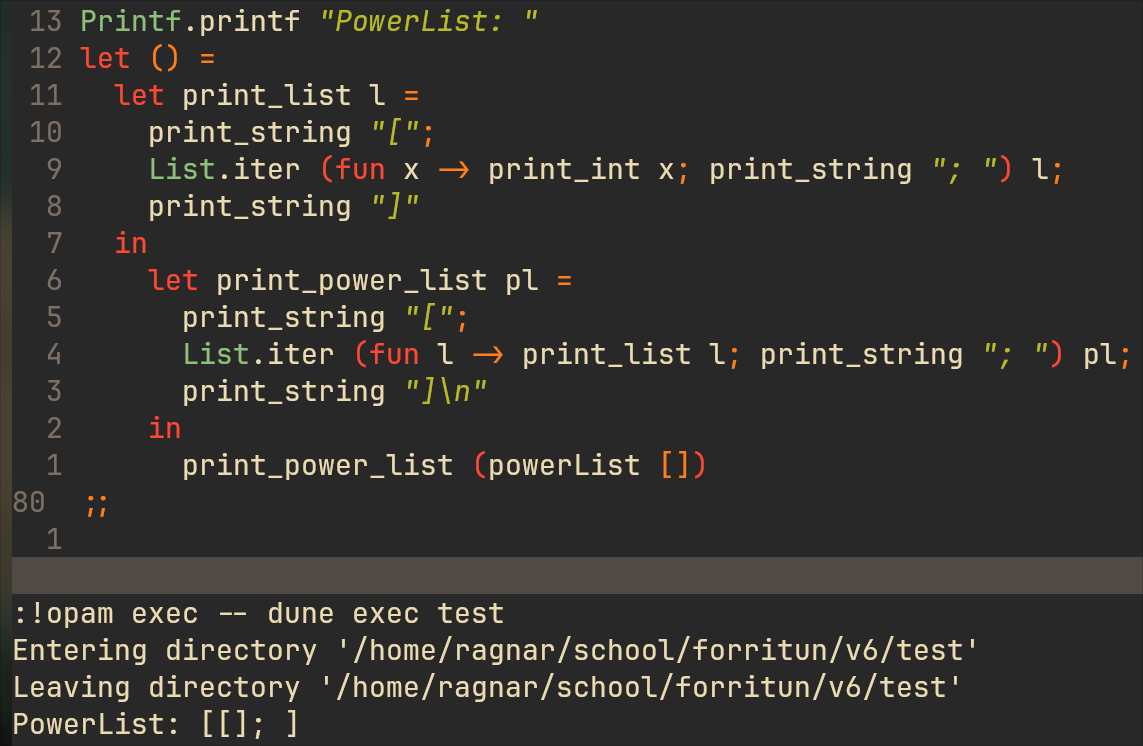
\includegraphics[scale=0.3]{powerlist2.png}
	\end{center}
\end{document}
